\documentclass[11pt]{article}

\usepackage{hyperref}
\usepackage{lipsum}
\usepackage{circuitikz}
\usepackage{graphicx}
\usepackage[margin=0.9in]{geometry}
\usepackage{setspace}
\usepackage{mathtools}
\newtagform{brackets}{[}{]}
\usetagform{brackets}

\title{Electronic Properties of Metals and Semiconductors, lab 1}
\author{Bijan Varjavand}
\date{due February 20 2017}
\begin{document}
\maketitle
\vspace{3.5in}
\section*{Abstract}
%\lipsum[1]
Four experiments were performed in this lab. The first was purely to recognize a correlation between voltage and current, a confirmation of Ohm's law. The data showed a slope, the resistance of the sample, of 1.68$\Omega$. The $r^2$ value of the linearization gave a result of 1, a perfect relationship that confirmed Ohm's law. The next experiment was done to find the conductivity of the sample, $\sigma$. Values of 1.73E7, 2.14E6, 2.61E7, 9.05E6, 5.21E6, and 7.76E7 S/m were obtained for brass, titanium, aluminum, bronze, steel, and copper respectively. The data deviated from literature values of 1.59E7, 2.4E6, 3.7E7, 8.7E6, 5.9E6, and 5.85E7 S/m by 8.1, 10.8, 29.3, 4.0, 11.7, and 32.6 percent, respectively. The third experiment was to find the linear thermal coefficient of resistivities for the same materials, yielding 2.0E-3, 6.2E-3, 3.9E-3, 3.1E-3, 1.9E-2, and 6.4E-3 $K^{-1}$, still in the same order as the above materials. These values deviated from literature values of 1.5E-3, 2.4E-5, 3.9E-3, 4.0E-3, 6.6E-3, and 4.3E-3 $K^{-1}$ by 33.3, 63.2, 0.0, 22.5, 97.1, and 49.2 percent, respectively. The final experiment simply showed relationships between temperature and conductivity in differently doped semiconductors.

\clearpage
\onehalfspacing
\section*{Introduction}
\ \ \ Laws and relationships of electrical properties such as voltage and conductivity help us understand the world around us. However, these laws are often complicated and vague, and often have limited applicability to the range of materials. Additionally, from an empirical point of view, just being shown an equation is not enough to trust the relationships given. Thus experimental confirmation of experiments such as Ohms law greatly enhances the learning and understanding of the student. Furthermore, additional relationships between variables which may not be obvious at first glance can be found during an experiment.\\

In order to understand useful equations and relationships, one first needs to understand the variables that are used in each equation. Thus, I will cover each of the variables mentioned in this lab report, explaining their significance. The variables used are related to circuits, which consist of electrons flowing through conductive materials. The flow of these electrons is able to generate work if it is taken advantage of properly.

\subsubsection*{Ohms Law}
\ \ \ Voltage can be thought of as an electric potential difference between two points in a circuit. It is the driving force that represents the strength of electron flow. The unit for voltage is the volt, V, equal to one Joule per Coulomb. This makes intuitive sense, as the number of joules per coulomb is simply the amount of work one can get done with a certain amount of charge. Current is related to the actual flow of the electrons. Its unit is the ampere, I, the flow of charge across a surface of one coulomb per second. Resistance, the final of the first 3 variables, is dependent on the properties and dimensions of the material that the electrons are flowing through. It is measured by how difficult it is to pass an electric field through a conductor. It is measured in Ohms, $\Omega$, with units derived from Ohms law – joules seconds per coulomb squared.\\

Variables such as voltage, current, and resistance are commonly interpreted in relation to circuits and electronic properties. This is taught in the form of Ohms law.
\begin{equation}
V = IR
\end{equation}

The relationships between voltage, current, and resistance are clearly shown. For example, if one increases resistance and holds current constant one can expect to see an increase in voltage. This also explains the units for an ohm, as it is simply voltage over current.

\subsubsection*{Resistance-Resistivity Relationship}
\ \ \ The next 3 variables are incorporated into an additional equation for resistance. These include length (L) and cross-sectional area (A). The third variable is resistivity, measured in ohm meters, an intrinsic value for each type of material. The concept of resistivity and its relationship it resistance becomes clearer after analysis of the relevant equation - the resistance-resistivity relationship. This is shown below.
\begin{equation}
R = \frac{\rho L}{A}, \rho = \frac{RA}{L}
\end{equation}

This equation makes it possible to find resistances of materials by simply knowing the dimensions and resistivity. One can think about this in terms of an obstacle course electrons have to pass through – where the resistivity is the difficulty of the course. A larger cross-sectional area will increase the space available for electron flow, and resistance will decrease. A longer length of the obstacle course will make it more difficult, increasing resistance. As a side note, one observes that resistivity is simply the inverse of conductivity - measured in Siemens per meter.
\begin{equation}
\rho = \frac{1}{\sigma}, \sigma = \frac{1}{\rho}
\end{equation}

\subsubsection*{Microscopic Model of Current}
\ \ \ The next series of variables are related to a more direct look at the particles that are related to current and electron flow. Looking closer, current is simply the random motion of electrons biased in a certain direction due to the electric field created by a voltage. J, the current density, is measured in amperes per square meter. It is utilized in the equation below.

\begin{equation}
J = \sigma E
\end{equation}

E, the electric field strength, is measured in Newtons per coulomb. We can see from this equation that, given an electric field of some strength E and the conductivity of the material $\sigma$, one can directly calculate the current density.\\

Another important property of a material is its mobility, $\mu$. This is calculated using the equation below. In this equation, $V_d$ is the drift velocity.

\begin{equation}
\mu = \frac{V_d}{E}
\end{equation}

The drift velocity of an electron can be thought of as the current. One needs to make this distinction to separate the drift velocity from the phase velocity, the actual speed of the electrons. The reason that these numbers are different is due to scattering and collisions in the material and between electrons. If one introduces the variable $n_e$, or n, as the number of electrons, one can simplify a few expressions to find an alternate equation for conductivity.
$$J = \sigma E$$
$$J = n_e V_d = n_e \mu E$$
\begin{equation}
\sigma = n_e \mu
\end{equation}

Here, The mobility of the material is now dependent on the number of electrons and conductivity, which still fits the model we have thus far described. We can summarize that mobility is a function of how densely scattering events occur, both temporally and spatially. This model persists by assuming that as long as an electric field persists, there will be a constant acceleration. Additionally, we assume electrons have a sort of inertia to them - once a field disappears, the electrons will keep drifting.

\subsubsection*{Semiconductors}
We see very different electronic properties in semiconductors compared to those of classic conducting metals. One way to approach these differences is by using the model we established above. The main approach is to compare the mobility of each material type. A metal has few impediments to electron flow, while semiconductors have fewer barriers and insulators have very densely packed scattering barriers. If one looks at the band gaps of the different materials, this becomes clear.
\begin{figure}[h]
	\centering
	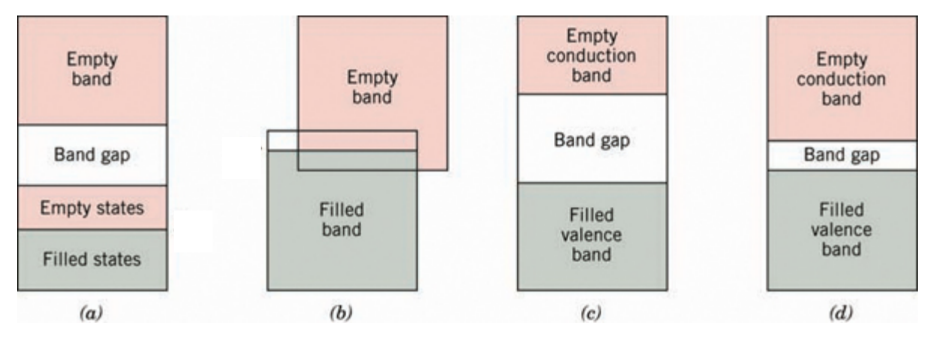
\includegraphics[scale=0.7]{bands.png}
	\caption{a-sample. b-conducting metal. c-insulator. d-semiconductor}
\end{figure}

The amount of energy required to move an electron from the valence to conducting band, known as the ionization energy, is either large, small, or 0 depending on the type of material. A useful benchmark to keep in mind is the average ionization energy of silicon, a classic semiconductor - 1.1eV. This relates to our model by associating the ionization energy with the density of scattering events - contributing to the mobility of the material. It also becomes clear that adding impurities would increase barriers and increase resistivity.\\

Intrinsic semiconductors can be doped by adding electron-rich or electron-poor regions in them. This creates n (electron rich) or p (hole rich) type semiconductors. This now extrinsic semiconductor has electrons or holes which artificially lower the band gap significantly, thus allowing for much higher conductivity. One can shift the ionization energies of semiconductors by doping them since electrons become more free. Doping converts the balanced numbers of holes and electrons in intrinsic semiconductors to a more skewed value depending on the type of doping. However, once these dopant electrons and holes are occupied, the material reverts back to its intrinsic semiconducting ionization energies.

\subsubsection*{Temperature Dependence}
\ \ \ The role of temperature in conductivity and resistivity now becomes clear both for metals and nonmetals. One can start analysis by observing band gaps and Matthiessen's Rule, shown below.

\begin{equation}
\rho = \rho_{thermal} + \rho_{imperfections} + \rho_{defects} = \rho_{thermal} + \rho_{residual}
\end{equation}

One can thus look at resistivity simply as contributions from imperfections and defects, and from temperature. The resistivity contributions from imperfections are obvious in metals - adding more imperfections increases scattering events and increases resistivity. Doping a semiconductor, while it introduces impurities, lowers the band gap by a large margin - resulting in a lower resistivity. The thermal resistivity for metals is relevant - as temperature increases the energy of the lattice and electrons increases. This generates more phonon interaction with the lattice, increasing resistivity. Increasing the temperature of semiconductors increases the number of charge carries, but decreases mobility in the same way.\\

A crucial equation for finding the change in resistivity in metals due to temperature is shown below, and is used for data analysis in this lab.

\begin{equation}
\rho = \rho_{ref}[1 + \alpha(T - T_{ref})]
\end{equation}

Where $\rho_{ref}$ and $T_{ref}$ are the reference initial values - our first data point pair taken. Usually this is at STP. $\alpha$ is the linear thermal coefficient of resistivity (in units of $K^{-1}$), unique to each material and which affects $\rho_{thermal}$. The implications of Matthiessen's Rule vary from material to material, as we will see later in the Results and Discussion section.

\section*{Procedure}
\subsubsection*{Lab 1a}
\ \ \ The first step was for us to prepare a sample of brass. We created a circuit with wires between a power supply, ammeter, and our sample. Additionally, we connected a voltmeter to our sample. This is shown below in \textbf{Figure 2}, in both physical and circuit form.

\begin{figure}[h]
	\begin{minipage}{.5\textwidth}
		\centering
		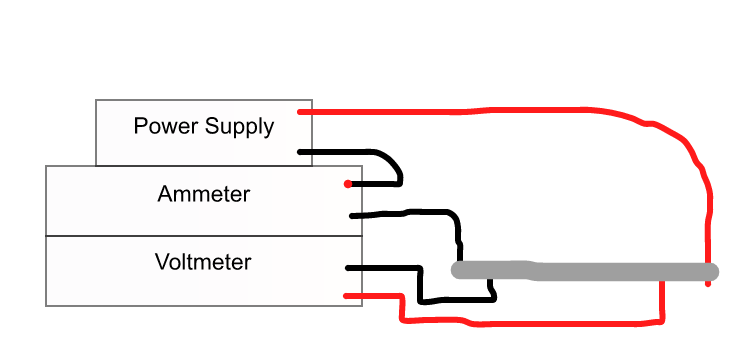
\includegraphics[width=\linewidth]{circuit1.png}
	\end{minipage}
	\begin{minipage}{.5\textwidth}
		\centering
		\scalebox{0.7}{
		\begin{circuitikz} \draw
		(0,0) to[battery] (0,4)
      		to[ammeter] (4,4) -- (4,0)
      		to[resistor] (0,0)
		(0.5,0) -- (0.5,-2)
      		to[voltmeter] (3.5,-2) -- (3.5,0)
		;
		\end{circuitikz}}
	\end{minipage}
	\caption{The physical and circuit-based representations of our setup for lab 1a}
\end{figure}

We simply varied the voltage on our power supply and measured the resulting change in current. For lab 1a part 2, we prepared additional samples of titanium and aluminum. While keeping current constant, we varied the distance between leads on our material to change the measured voltage (for each material).\\

\subsubsection*{Lab 1b}
\ \ \ For lab 2a, we created a circuit as shown above, but placed the sample (resistor) into a furnace, connecting all necessary components to leads coming out of the furnace. Additionally we attached a thermocouple, wrapping it around the sample. This was to measure voltage, which we can convert to temperature. The integrated labview software is able to generate the necessary data, and automatically does all the conversions we need. A diagram of this setup is shown below in \textbf{Figure 3}. The circuit elements are the same besides the thermocouple.

\begin{figure}[h]
	\centering
	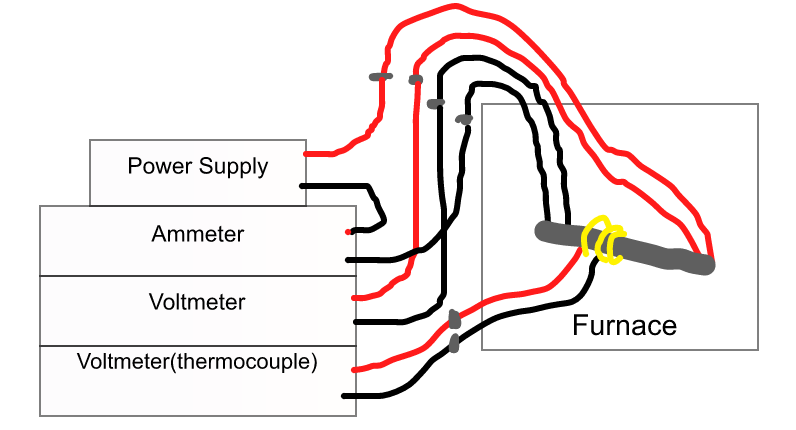
\includegraphics[scale=0.5]{circuit2.png}
	\caption{Our second setup, in a furnace with a thermocouple}
\end{figure}

\subsubsection*{Lab 1c}
\ \ \ We started with a silicon wafer, with a layer of titanium and copper on top of one side. This is to allow a conductive surface - the titanium acts as a way to more strongly bind the copper and silicon. We then added a photoresist, a polymer which absorbs radiation, on top of the wafer. Putting a mask on the photoresist let us break down the unmasked section with uv rays. We then washed off the photoresist and dried the wafer. Then we dissolved the exposed copper, washed and dried, then dissolve the titanium, and washed and dried. We then removed the photoresist, washed, and dried the wafer.\\

Once back in the lab, we scribed lines across our wafer to ease breaking it. Breaking our wafer along these scribed lines was not uneventful as the wafer was incredibly thin and fragile. Unfortunately our wafer broke along the middle. We then repeated what we did in lab 1b, connecting everything to the exposed copper to measure the conductivity across the silicon wafer.

\section*{Results and Discussion}
\subsubsection*{Verifying Ohm's Law}
\ \ \ Intuition about plotting the data from our experiment in part 1 of lab 1a was created by rearranging Ohm's law, shown below.
\begin{equation}
V = RI
\end{equation}
This new equation, derived from \textbf{Equation 1}, arranges Ohm's law into a linear relationship, where voltage is equal to the dependent variable I times the constant R. We see in the data below in \textbf{Figure 4} to be a verification that we expect the slope of this data to be R.

\begin{figure}[h]
	\centering
	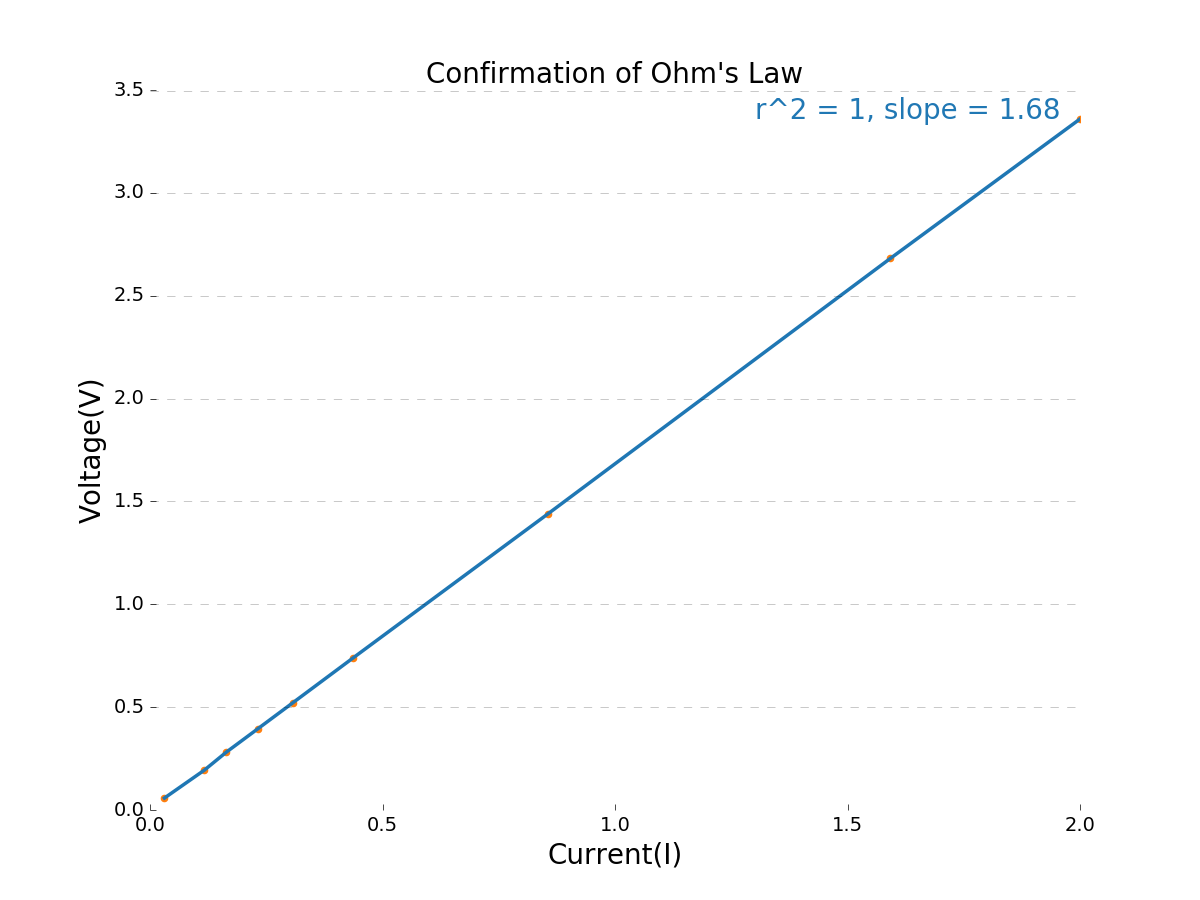
\includegraphics[scale=0.35]{ohmslaw.png}
	\caption{Using $V = RI$, where R is the slope of this line}
\end{figure}

The resistance of the material is measured to be 1.68. However, this value can not be compared to any literature values to the wide array of variables that affect resistance. We can, however, use this to verify the accuracy of Ohm's law. One only needs to glance at the plot to see how perfectly each point fits on the line. Furthermore, the $r^2$ value of the linear regression is 1! That is a 100\% accuracy of fit. This makes sense, as the direct relationship between voltage (the driving force for electron flow), and current (the speed of electron flow), is obvious from an intuitive point of view.

\subsubsection*{Length Dependence of Resistance}
\ \ \ In order to calculate the length dependence of resistance, we need to manipulate \textbf{Equation 2}, the resistance-resistivity relationship. Incorporating it into Ohm's law gives us a form which is plottable.
$$R = \frac{\rho L}{A}, V = RI$$
\begin{equation}
V = \rho \left(\frac{IL}{A}\right)
\end{equation}

With this equation we just need to plot voltage versus current length over cross-sectional area in order to find the slope, the resistivity of the material. Linearizing the data points gives us some degree of confidence which we can ascertain resistivity values from. The plot is shown below in \textbf{Figure 5}.

\begin{figure}[h]
	\centering
	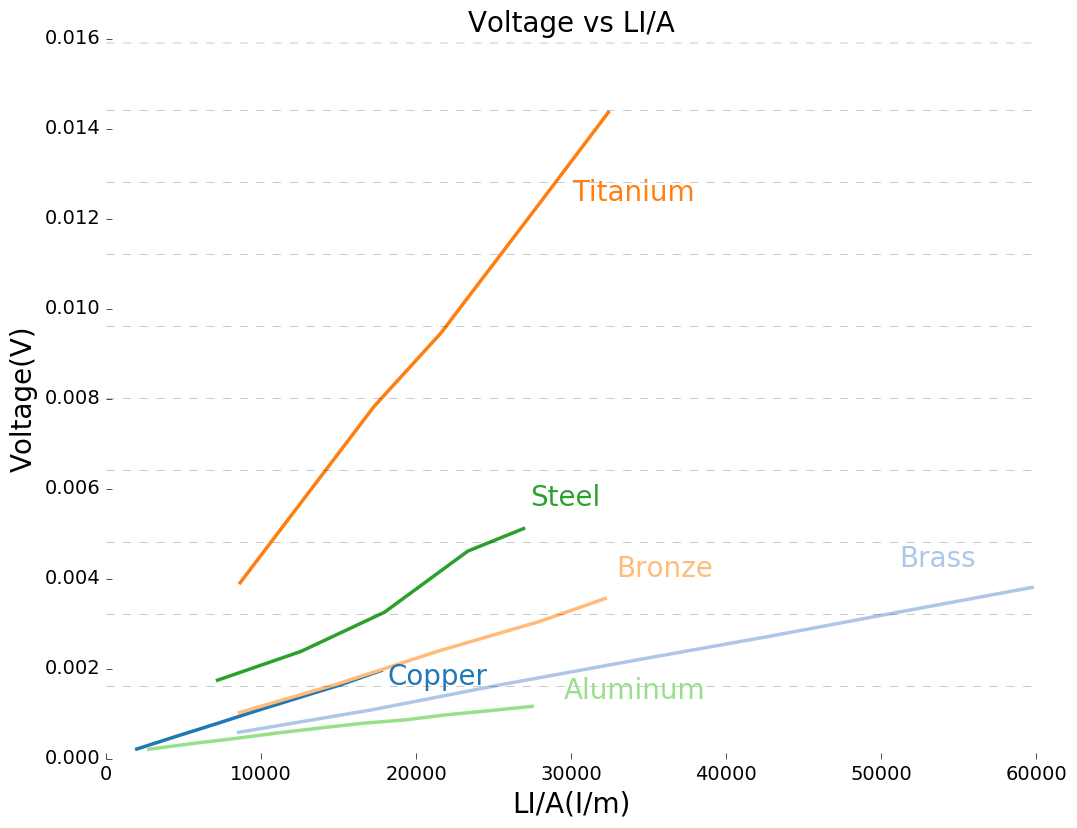
\includegraphics[scale=0.35]{resistivity.png}
	\caption{Resistivity values (the slope) for 6 different metals}
\end{figure}

Important relationships given in \textbf{Equation 2} are finally replicated empirically in \textbf{Figure 5}. All the metals are clearly following a direct, first-order relationship. This mirrors what we expect in \textbf{Equation 10}.\\

We trust our values and the linear relationship of our lines because the entire x-axis, $\frac{IL}{A}$, is held constant at each value. The linear regressions of each line were calculated and compared to literature values. This is all documented in \textbf{Table 1}. The errors are within expected margins, as the sources of error include only error from measurement of the length of our material as well as the multimeter measurements. This is because the measurement was done with an low accuracy of centimeter tick marks on a meter stick. Additionally, the values of current and voltage were constantly fluctuating slightly, introducing slightly more error.

\subsubsection*{Temperature Dependence of Conductivity in Metals}
\ \ \ In order to organize the data of temperature and resistance in metals, we used \textbf{Equation 8}. Manipulating equations gives us a more straightforward linearizable version shown in \textbf{Equation 11}, utilizing \textbf{Equation 3} to convert from resistivity to conductivity.
$$\alpha = \frac{1}{\rho}\frac{\rho - \rho_{ref}}{T-T_{ref}}$$
\begin{equation}
\alpha = \sigma\frac{\rho - \rho_{ref}}{T-T_{ref}}
\end{equation}

Using the data that was given to us by the LabView software lets us generate \textbf{Figure 6}, shown below.

\begin{figure}[h]
	\centering
	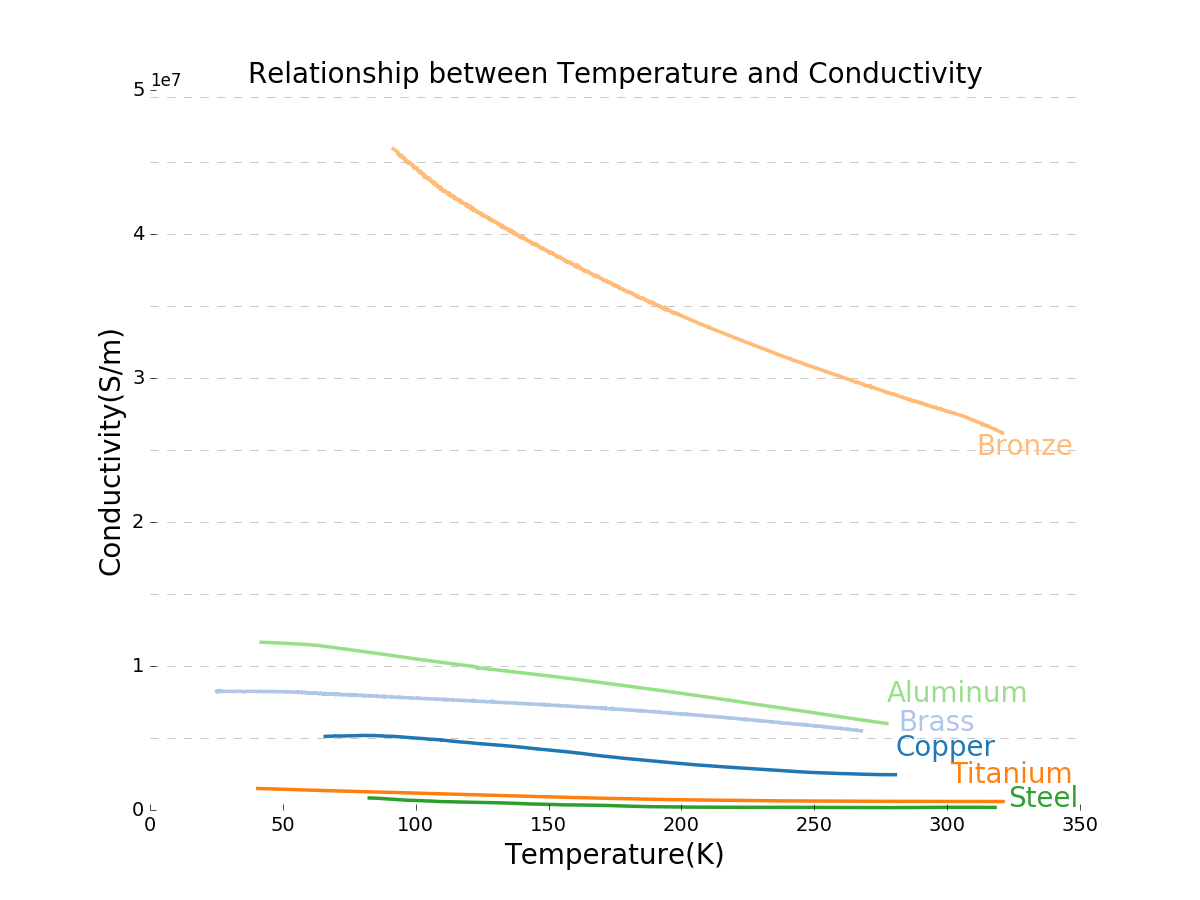
\includegraphics[scale=0.35]{lab1b.png}
	\caption{Linear thermal coefficient of resistivity (slope) for 6 different materials}
\end{figure}

\textbf{Figure 6} shows the wide range of conductivities across different materials. The general trend to observe is the downward trend of the data. This is due to the $\rho_{thermal}$ in Matthiessen's Rule. The difference between materials themselves is due to the contribution of $\rho_{imperfections}$ which is unique to the specific state of each material. To explain the downward trend and low value of $\alpha$, we observe \textbf{Equations 4, 5, and 6}. This describes the model we created earlier for microscopic properties of current. Specifically looking at \textbf{Equation 5}, we can see how the drift velocity of the material is affected by the mobility of the material. Increasing temperature excites the lattice and number of scattering events. This increases the collisions and lowers the drift velocity, decreasing conductivity (seen explicitly in \textbf{Equation 5}).\\

The slopes of each line were again calculated with linear regressions, and the values (linear thermal coefficient of resistivity) are all shown in \textbf{Table 2}. The literature value deviations are also included in \textbf{Table 2}, and out percent errors are within expectation except for two materials - phosphor bronze and steel. The sources of error for this experiment are the same as the previous experiment, with additional sources of error included in the thermocouple. The addition of a thermocouple introduces high amounts of error since the contact point between the thermocouple and the material needs to be firm to be reliable. Getting this strong connection is very challenging. This must have been the problem with steel - a weak connection somewhere in the circuit or in the thermocouple.

\subsubsection*{Temperature Dependence of Conductivity in Semiconductors}
\ \ \ The results from our experiment measuring the thermal coefficient of resistivity for semiconductors were generated in the same way as with metals - utilizing \textbf{Equation 11}. The data is shown below in \textbf{Figure 7}.

\begin{figure}[h]
	\centering
	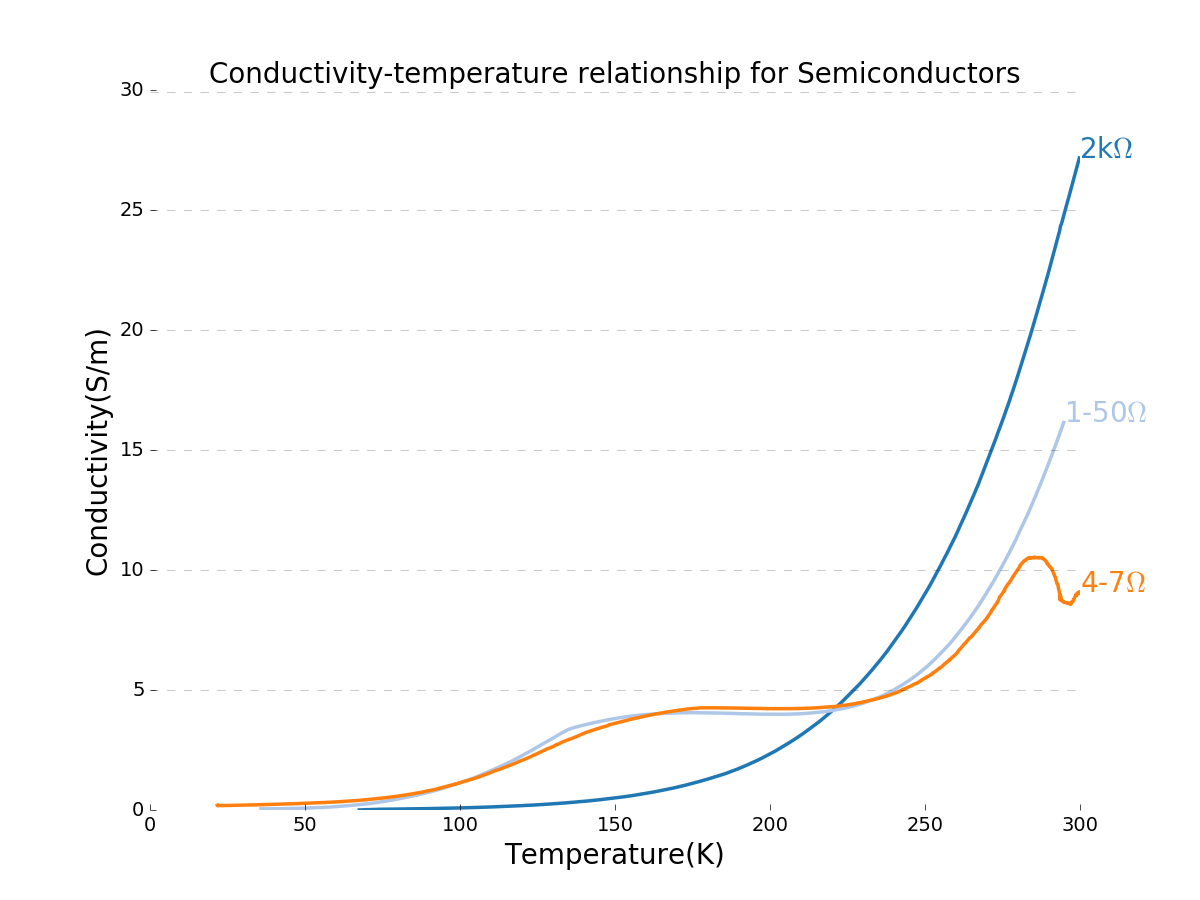
\includegraphics[scale=0.35]{semiconductors2.png}
	\caption{Conductivity-Temperature relationship for different semiconductor doping}
\end{figure}

The exact value of the linear coefficient of thermal resistivity is hard to determine for semiconductors. This is due to what we described in \textbf{Equation 7} - Matthiessen's Rule. The different resistivity (and thus conductivity) contributions from scattering, electron hole pair creation, impurities, and dopant effects give mixed results for a final value. The scattering and impurity contributions are the same as in metals, affecting the mobility of the material as described above for \textbf{Figure 6}. These, however, play less of a role than the contributions from dopant effects and the associated electron hole pair addition. This is why we see the 4-7 and 1-50 $\Omega$ semiconductors have a higher conductivity initially.\\

However, once a certain thermal value is reached, all of the dopant electrons and holes will be used up and the material's band gap will revert to its intrinsic state. Yet one can't forget the presence of the dopant materials still in our semiconductor. These contribute to the resistivity by hindering electron flow though the lattice. This is represented in \textbf{Figure 7} by the plateauing of the highly doped semiconductors and by the surpassing conductivity of the low or non-doped 2k$\Omega$ semiconductor.\\

The main error in this portion of the lab consists of the dipping of the 4-7$\Omega$ semiconductor at the end, which can be attributed to either a random bump disturbing the leads or the leads degrading due to the high temperature. Degradation of the leads seems more likely as we have already discarded conductivity data above 300K due to lead degradation.

\subsubsection*{Additional Analysis: Bigger Picture}
One can fix this issue, as well as generate additional inferences about the data, by plotting all our resistivity data on a log axis. This is shown below in \textbf{Figure 8}.

\begin{figure}[h]
	\centering
	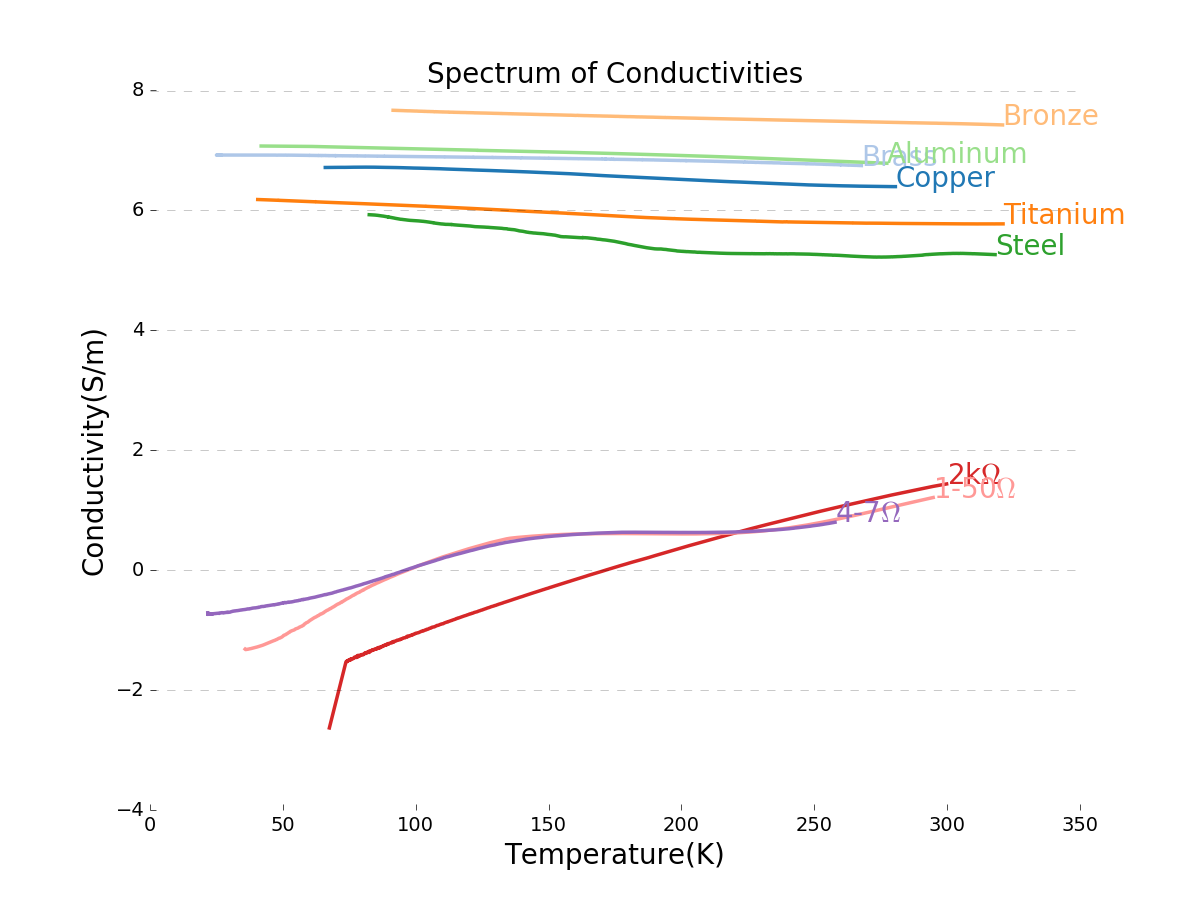
\includegraphics[scale=0.35]{allmats.png}
	\caption{All our materials with their $log_{10}$(resistivity) vs temperature plotted simultaneously}
\end{figure}

It becomes clear that the main differences between these materials has nothing to do with Matthiessen's Rule, or at least are not affected by a noticeable magnitude. The clear difference between the categories of materials is related to \textbf{Figure 1}. The band gap differences between classes of material are much greater than in between the small thermal laws. Another important variable to consider is the linear coefficient of thermal resistivity. One can see right away how the slopes of these groups are very different from each other. This definitely puts the intricate effects we have been observing into perspective and clarifies many concepts by giving an overview of the entire spectrum of materials.

\clearpage
\section*{Appendix}

\begin{table}[h]
	\centering
	\begin{tabular}{||c|c|c|c||}
	\hline
	Material & Data & Literature & \% Error\\
	\hline
	\hline
	Brass & 1.73E7 & 1.59E7 & 8.1\%\\
	\hline
	Titanium & 2.14E6 & 2.4E6 & 10.8\%\\
	\hline
	Aluminum & 2.61E7 & 3.69E7 & 29.3\%\\
	\hline
	Bronze & 9.05E6 & 8.7E6 & 4.0\%\\
	\hline
	Steel & 5.21E6 & 5.9E6 & 11.7\%\\
	\hline
	Copper & 7.76E7 & 5.85E7 & 32.6\%\\
	\hline
	\end{tabular}
	\caption{Conductivity literature value comparisons}
\end{table}

\begin{table}[h]
	\centering
	\begin{tabular}{||c|c|c|c||}
	\hline
	Material & Data & Literature & \% error\\
	\hline
	\hline
	Brass & 2.0E-3 & 1.5E-3 & 33.3\%\\
	\hline
	Titanium & 6.2E-3 & 2.4E-5 & 63.2\%\\
	\hline
	Aluminum & 3.9E-3 & 3.9E-3 & 0.0\%\\
	\hline
	Phos Bronze & 3.1E-3 & 4.0E-3 & 22.5\%\\
	\hline
	Steel & 1.9E-2 & 6.6E-3 & 97.1\%\\
	\hline
	Copper & 6.4E-3 & 4.3E-3 & 49.2\%\\
	\hline
	\end{tabular}
	\caption{Linear thermal coefficient of resistivity literature value comparisons}
\end{table}

\subsubsection*{References}

\ \ \ 1. PBR Phosphor bronze ribbon. Tokyo Resistance Wire Co. Ltd. Web site. \url{http://main.tokyo-resistance-wire.com/en/products/pbr.html}. Updated 2017.\\

2. Titanium (ti) material information. Goodfellow Web site. \url{http://www.goodfellow.com/E/Titanium.html}.\\

3. Properties table of stainless steel, metals and other conductive materials; \url{http://www.tibtech.com/conductivity.php} Web site. . Accessed 2/20/, 2017.\\

4. Temperature coefficient of resistance. Resistor Guide Web site. \url{http://www.resistorguide.com/temperature-coefficient-of-resistance/}. Accessed 2/20/, 2017.\\

5. The Engineering Toolbox. Resistivity and conductivity - temperature coefficients for common materials. \url{http://www.engineeringtoolbox.com/resistivity-conductivity-d_418.html} Web site.

\end{document}